\chapter{Results}
\label{chap:results}
%Merk at vi egentlig mener at diskusjonen i seg selv er en del av resultatet! Bruk diskursjon som et underpunkt til resultat

\begin{comment}
\section{Results from the Spectrometer I} 
the wave spectrum from one of the types. This can be compared to the associated colors wave spectrum. 
\section{Results from the Spectrometer II}
Comparing the signature of two different types of plastic (de gjennomsiktige pelletsene), which more or less have the same signature
\section{Principal Component Analysis I}
Using the different types of plastic only

\section{Principal Component Analysis II} 
The plastic types compared with algae

\section{The Final Method} 
\end{comment}

\section{PCA - Introduce and discuss figures}
The results from the PCA of the measurements showed no clear clusters or trends that would make it possible to distinguish individual types of plastic at this stage. The plot below shows the principal component analysis done on the results from scanning the plastic samples using hyper spectral imaging. The horizontal axis of the plot shows the first principal component and the percentage of the variables it explains, while the vertical axis shows the second principal component and its percentage for explained variables. The rings around clusters with the same color, or samples of the same type, are the 95\% confidence interval of the type, i.e. 95\% of the samples should lie within the ring. These should therefore clearly indicate whether there are any clusters depicting patterns in the sample data. Finally, the colored arrows on the circle centered in (0, 0) depict the direction of the increasing level of that color. The following along the direction indicated by the red arrow shows an increasing level of the color red in the sample, while following the blue arrow shows an increasing level of the color blue etc.The tested variables were previously presented in the \textit{Method} section.

\subsection{PCA with all Plastic Samples}
Figure \ref{fig:PCA_plastics_full_doub_cont} shows the contributions from the different wave lengths to the two principal components. The horizontal axis represent the wave lengths and the vertical axis the contribution in percent. The dashed red line represent 0.253\% or the line that shows the exact equal contribution from all wavelengths. Integrating the line would result in $0.253\% \cdot (700 - 400)/(0.758) \approx 100\%$.%Dette er feil. det skal være 0.252 siden det er en måling hver 0.758 og ikke hver nanometer, så er det mer riktig på bildet.
Also, the color of the line depicts the color at that wavelength, the blue color of the line at 450 nm is the color of light with that specific wavelength. 
\\\\%Påpeke at selv der man ser clusters så er ikke dette fremtredende i den samme plasttypen, men heller på bakgrunn av den fargen plasten innehar. 
As can be seen in the plot in figure \ref{fig:PCA_plastics_only_full_scat}, PC1 accounts for over 90\% of the variance. From the signature and contribution of PC1 in figure \ref{fig:PCA_plastics_full_doub_cont} it is apparent that the 94.1\% descriptive property of the first principal component is not rooted in one wave length or in a combination of wave lengths. The even distribution over the spectrum visualize the fact that PC1 mainly describes the \textit{lightness} of the plastic. From the position of the different samples it is clear that the results are dominated by this fact. Due to the low variance of the second principal component, of only X \%, the vertical spread and thus the few clusters there are are not well described and may not be deemed representative.

\begin{figure}[H]
    \centering
    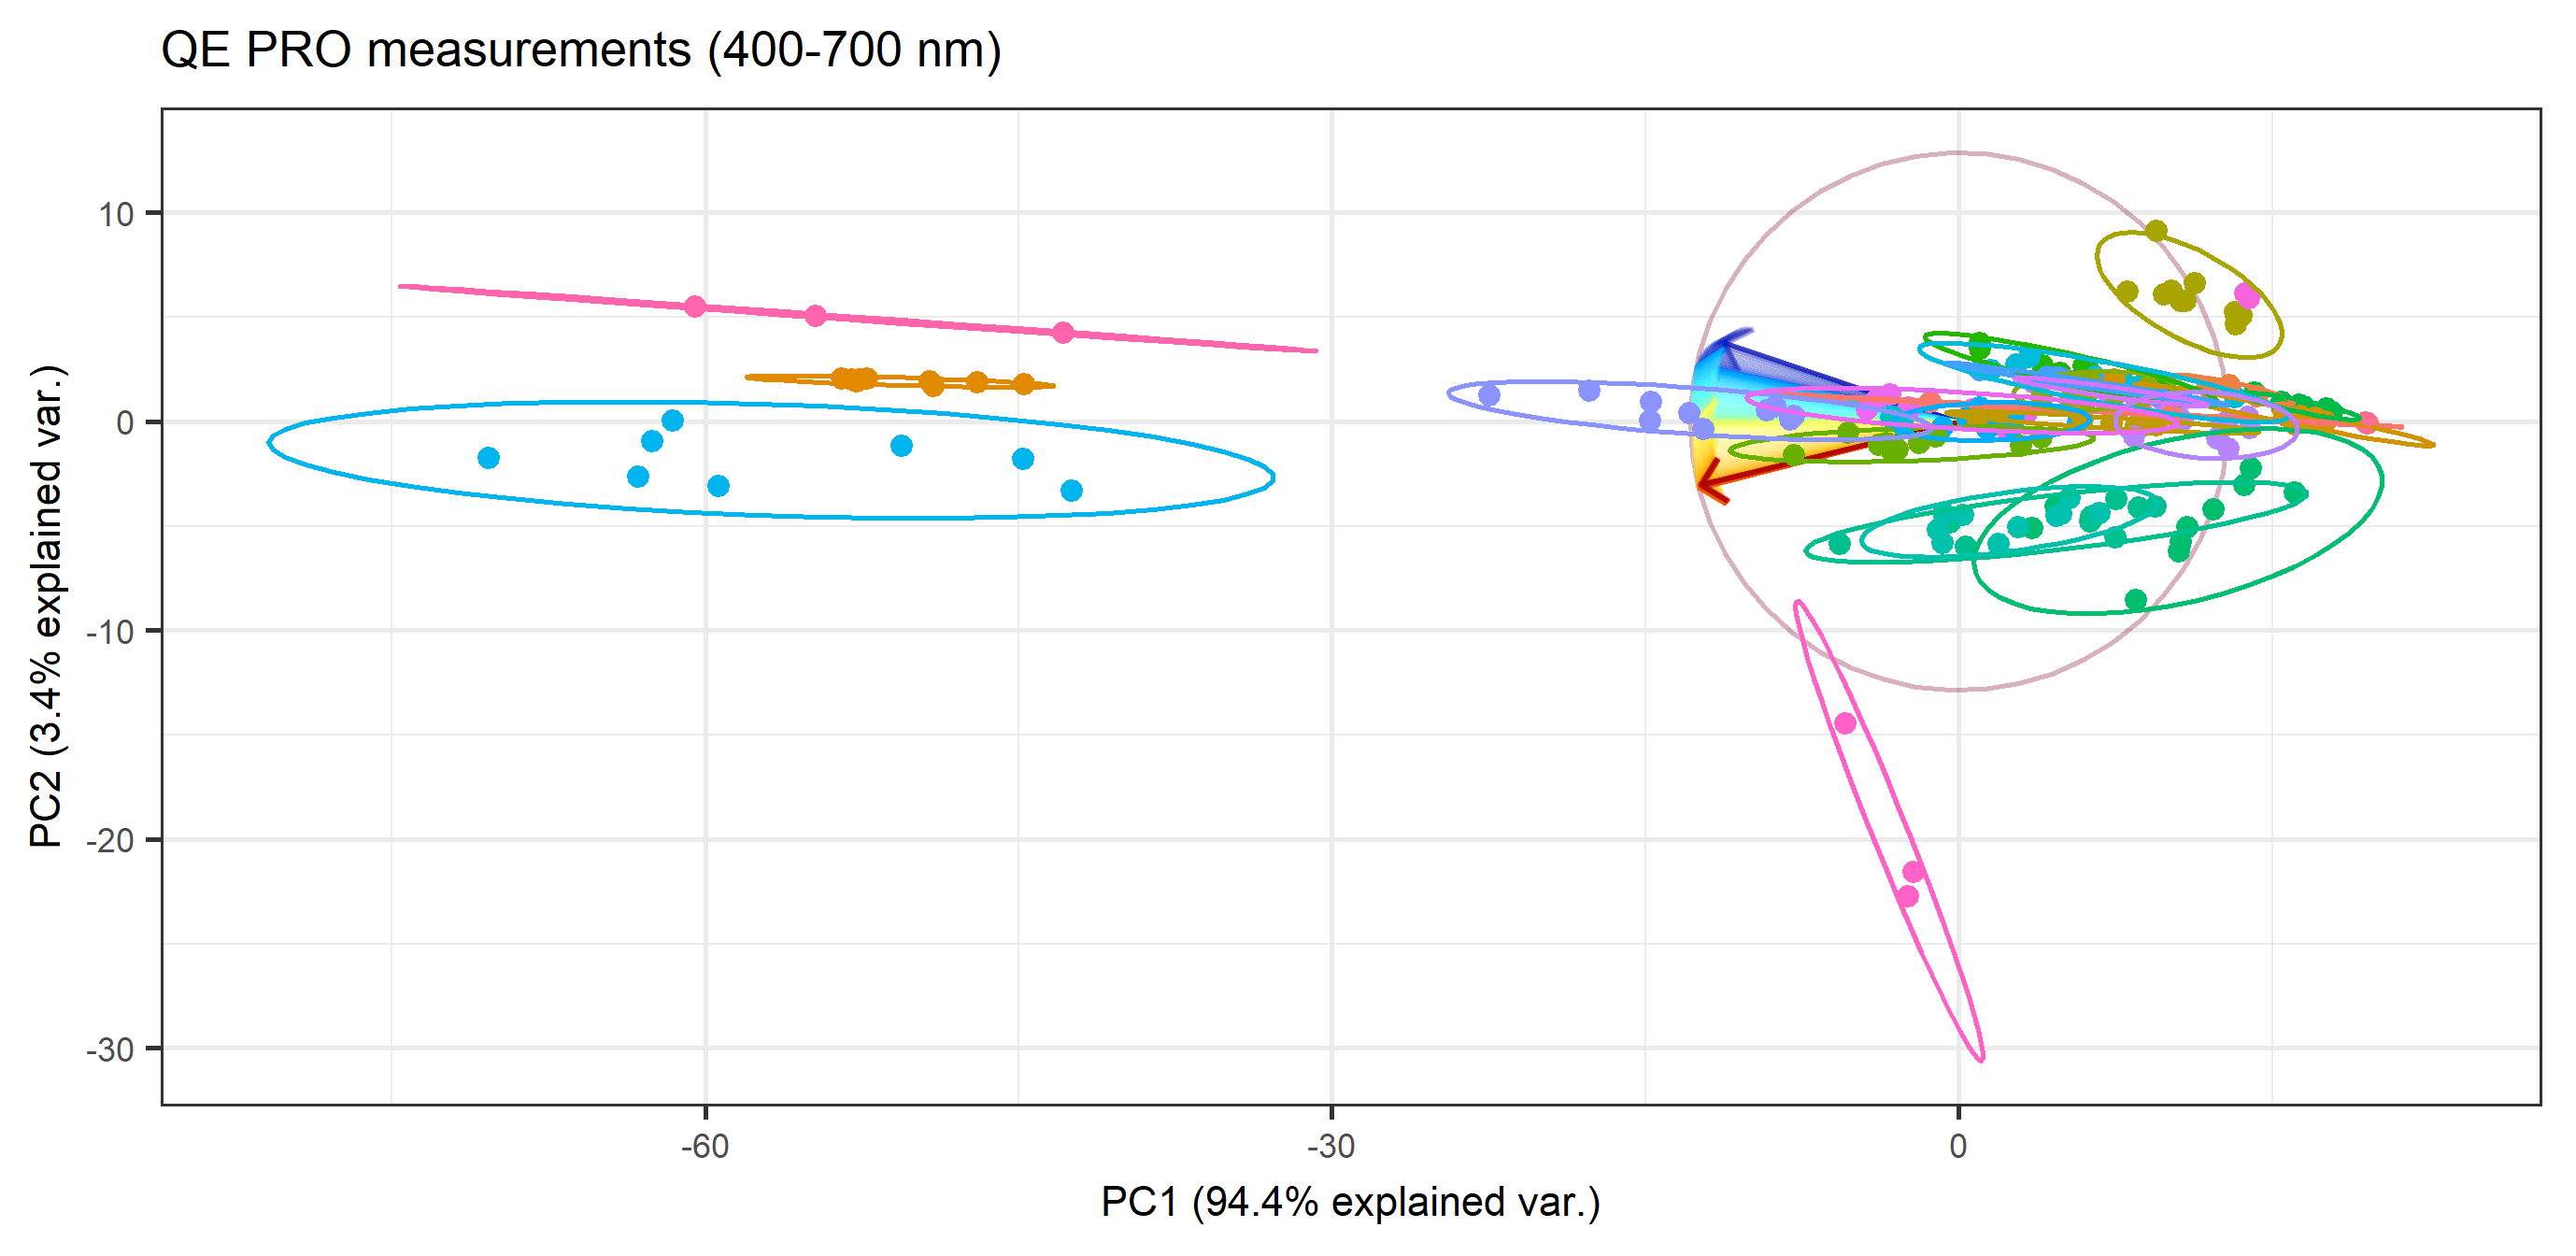
\includegraphics[width=1\textwidth]{Images/results/PCA_plastics_full_only_scat.png}
    \label{fig:PCA_plastics_only_full_scat}
    %\caption{Scatter plot of the results of the PCA with all plastic samples.}
    \caption{Scatter plot of the results of the PCA with all plastic samples}
\end{figure}


\begin{figure}[H]
   \centering
    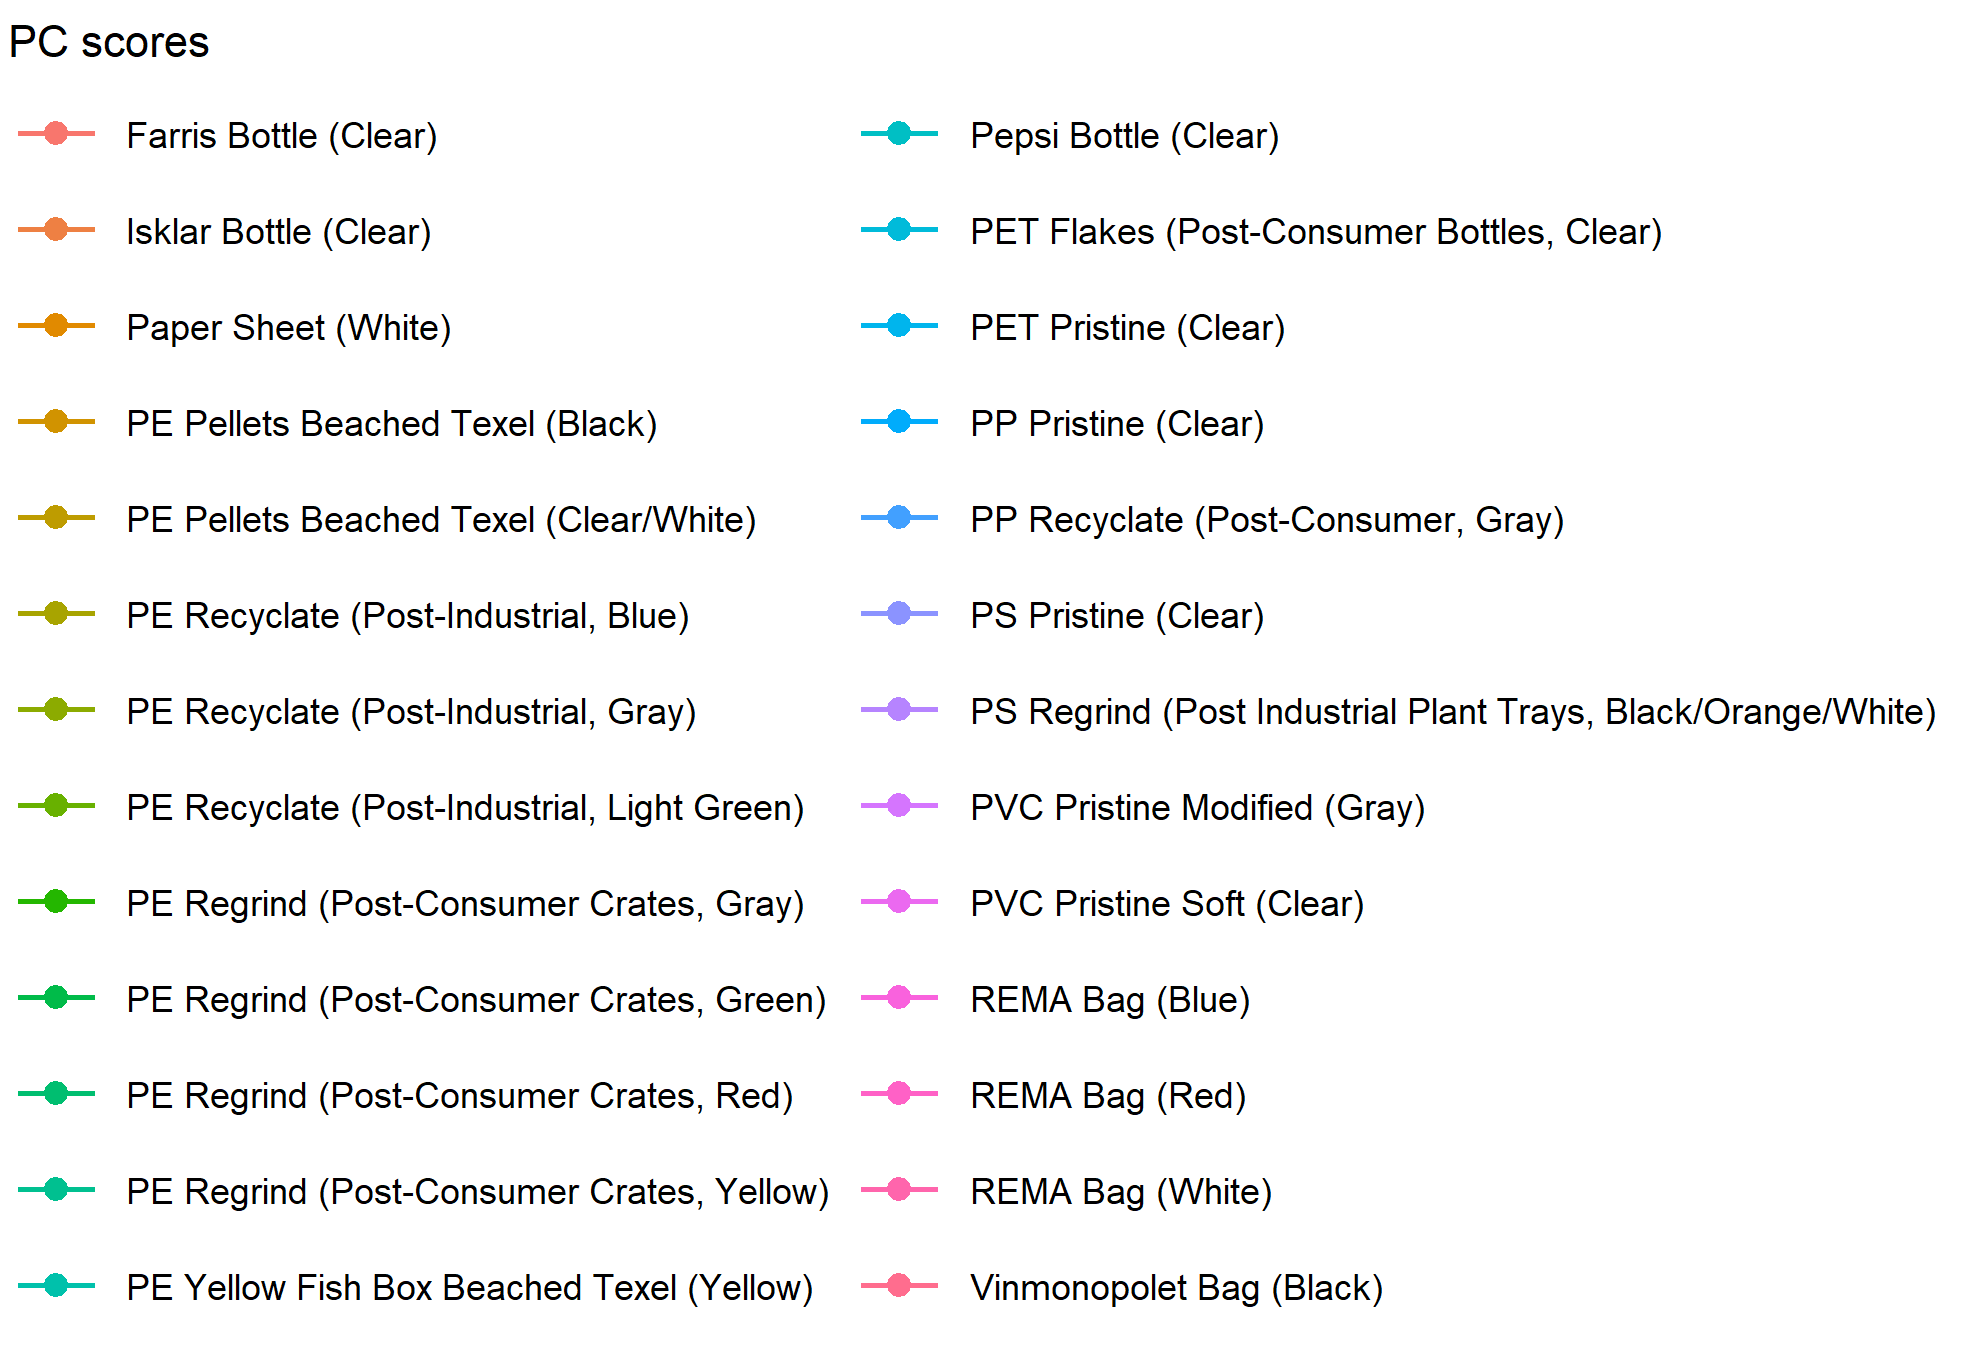
\includegraphics[width=0.7\textwidth]{Images/results/PCA_plastics_full_list.png}
  \caption{List of all scanned plastic samples and their respective colors.}
  \label{fig:PCA_plastics_full_list}
\end{figure}

\begin{figure}[H]
    \centering
    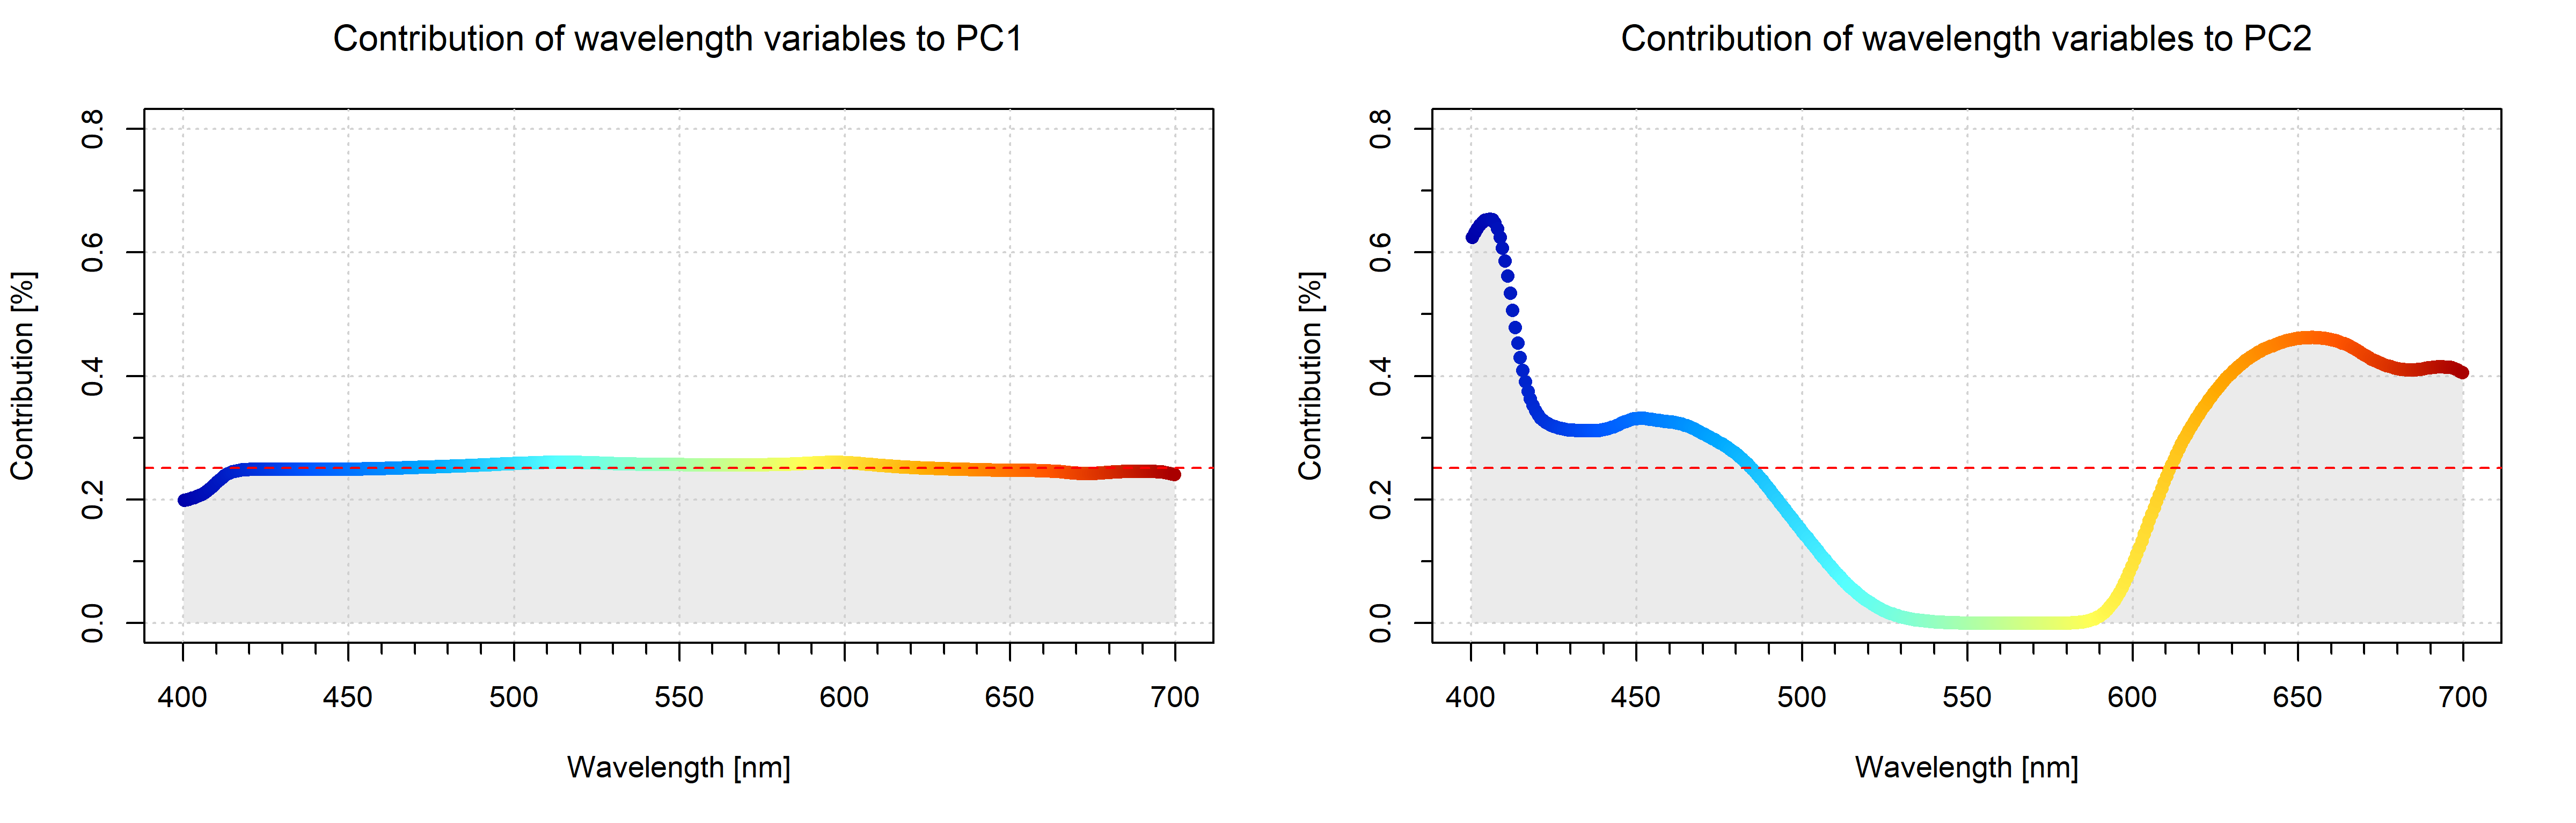
\includegraphics[width=1\textwidth]{Images/results/PCA_plastics_full_doub_cont.png}
    \caption{Contribution plot of the results of the PCA with all plastic samples.}
    \label{fig:PCA_plastics_full_doub_cont}
\end{figure}

\subsection{PCA with Reduced Plastic Samples}
However, despite the lower explanation percentage of PC2, there are clusters. These are quite apparent in the top and bottom of the scatter plot in figure \ref{fig:PCA_plastics_reduced_only_scat}. The issue arise when comparing these clusters to their respective plastic type. There are no other clear clusters related to these types of plastic. The clear clusters these types are a part of are based on the color of the plastic and not inherent properties of the material. The bottom cluster consists of PE Recyclate of the color blue together with samples from the blue in the logo on a plastic bag. Similarly, the top cluster consists of PE Regrind and PE Yellow Fish Box Beached Texel, both of which are yellow in color. It is therefore difficult to argue that these clusters indicate anything other than the color additives in the material.
\\\\
%Tenke på å markere clusterene med tall, slik at det blir lettere å omtale
Based on the tendency of the clear plastic to be on the left side of the cluster on can assume that the white paper background have had an impact on the results, and subsequently on the principal components. The samples of PS Pristine were particularly clear, as may be seen in the \textit{Materials} subsection of \textit{Methods}. Given that these are the main contributions to the spread along the horizontal axis, one could argue that without the light background, the lightness and clearness of the material would be less prominent in the first principal component. This would possibly further change the composition of the principal components and subsequently change the patterns on the scatter plots. 
\\\\%Snakke med Asgeir om dette og høre hva han tenker om at papiret har påvirket resultatene og at vi i utgangspunktet ikke har tid til å tilbringe en hel ny dag på laben for å teste på nytt. Aksel har gjort tester tidligere der han har fått samme resultat med at "lysheten" til prøvene har hatt stor innvirkning
The contribution plot of the second principal component does show that the lower end of the spectrum has ha larger impact than the larger wavelengths. 

\begin{figure}[H]
    \centering
    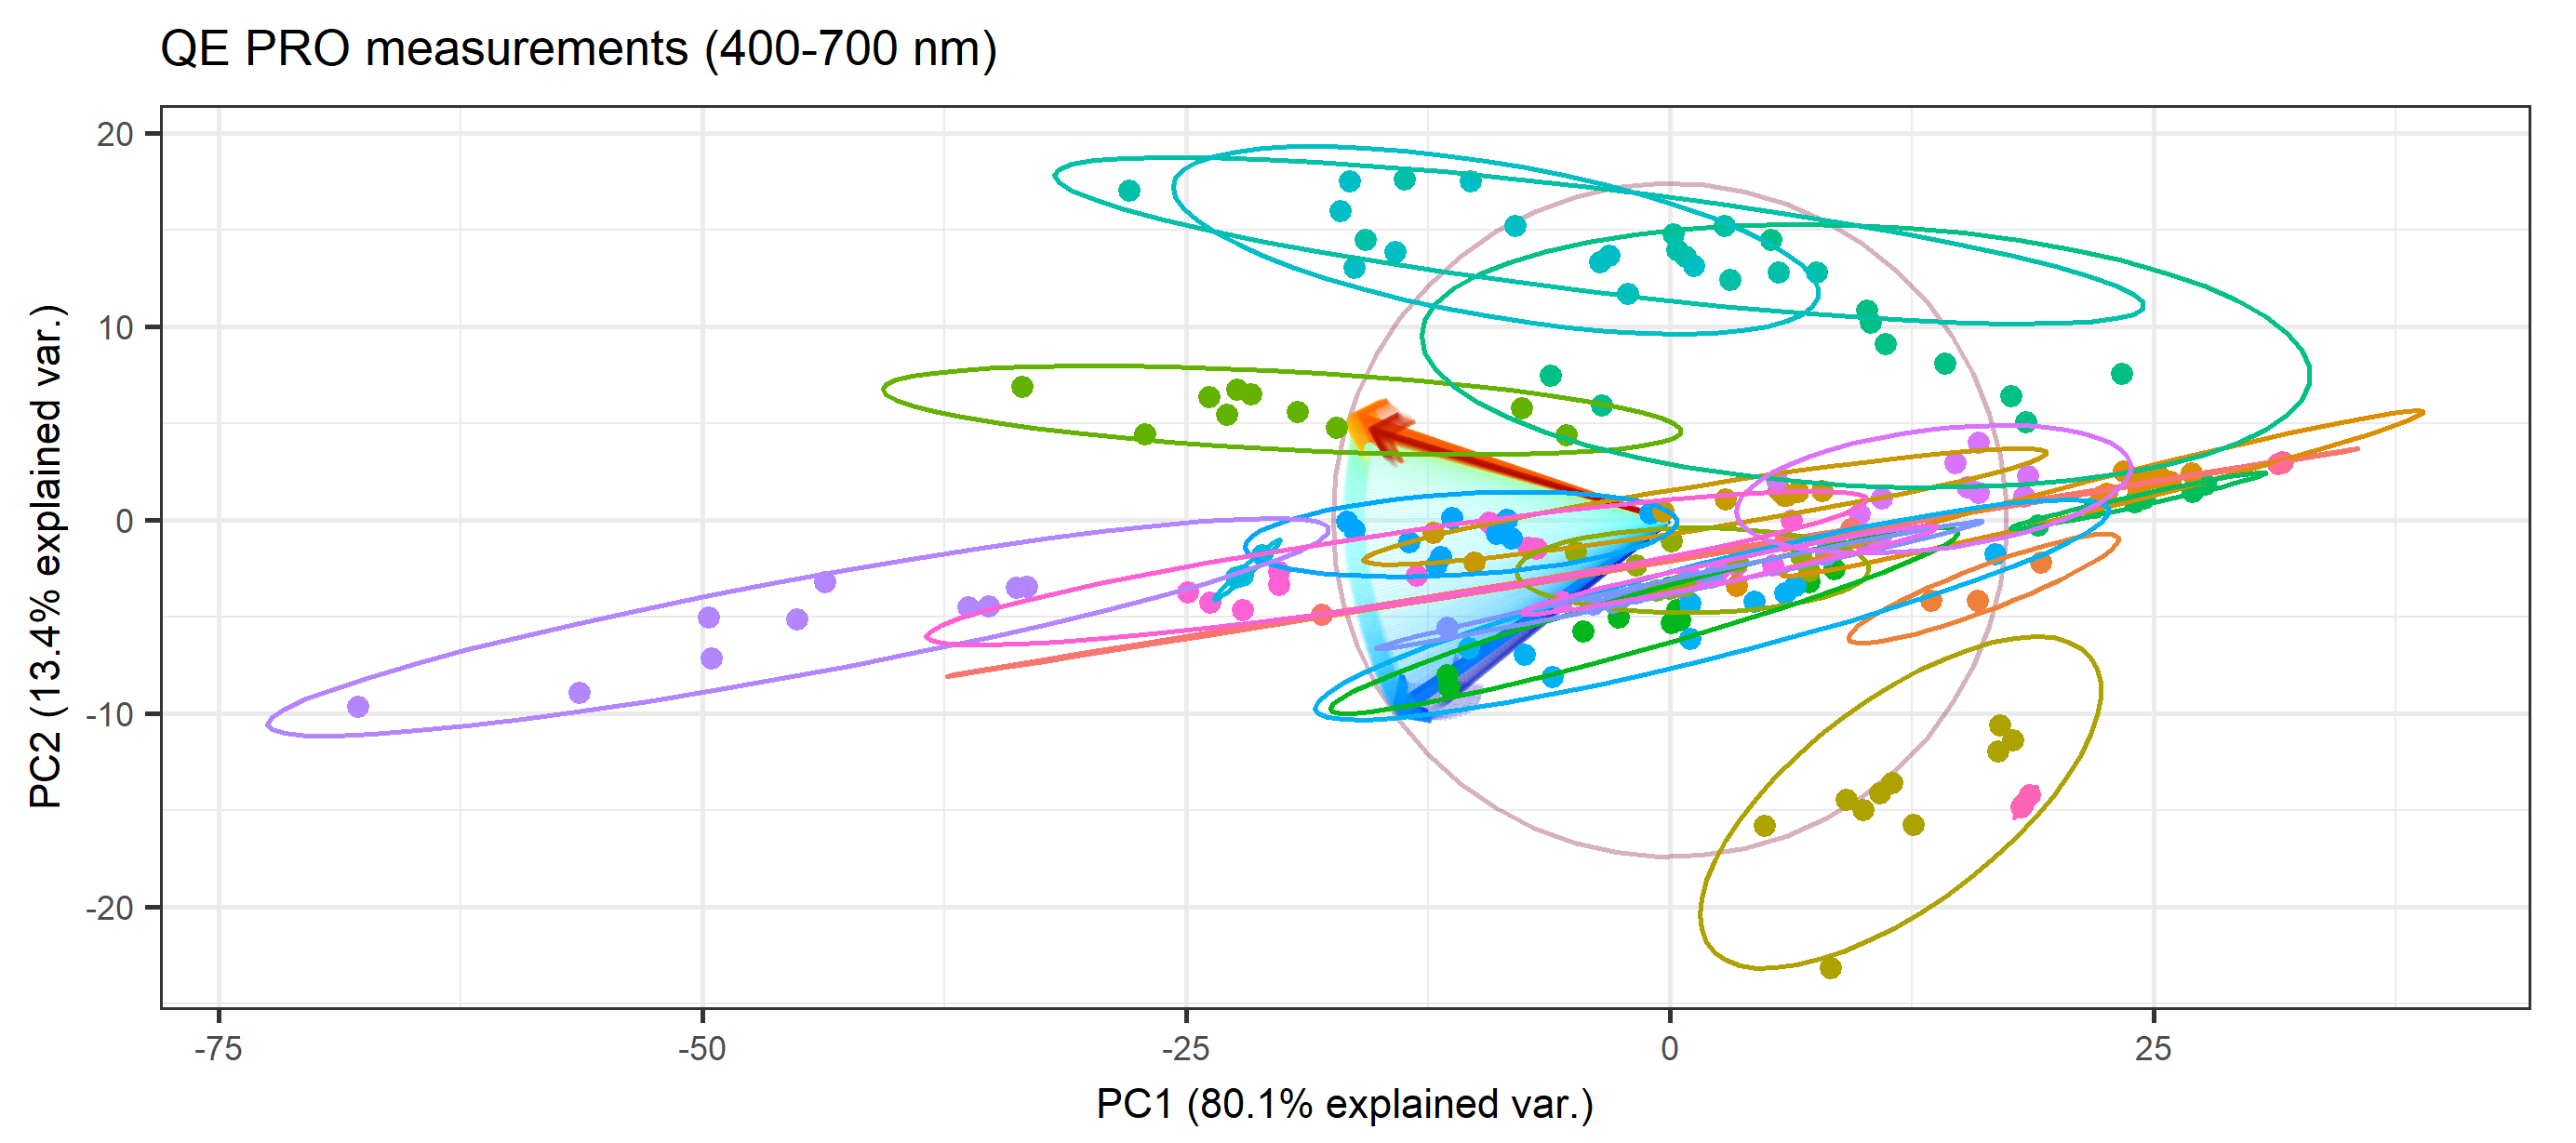
\includegraphics[width=1\textwidth]{Images/results/PCA_plastics_reduced_only_scat.png}
    \caption{Results of the PCA with reduced Plastic Samples}
    \label{fig:PCA_plastics_reduced_only_scat}
\end{figure}

\begin{figure}[H]
    \centering
    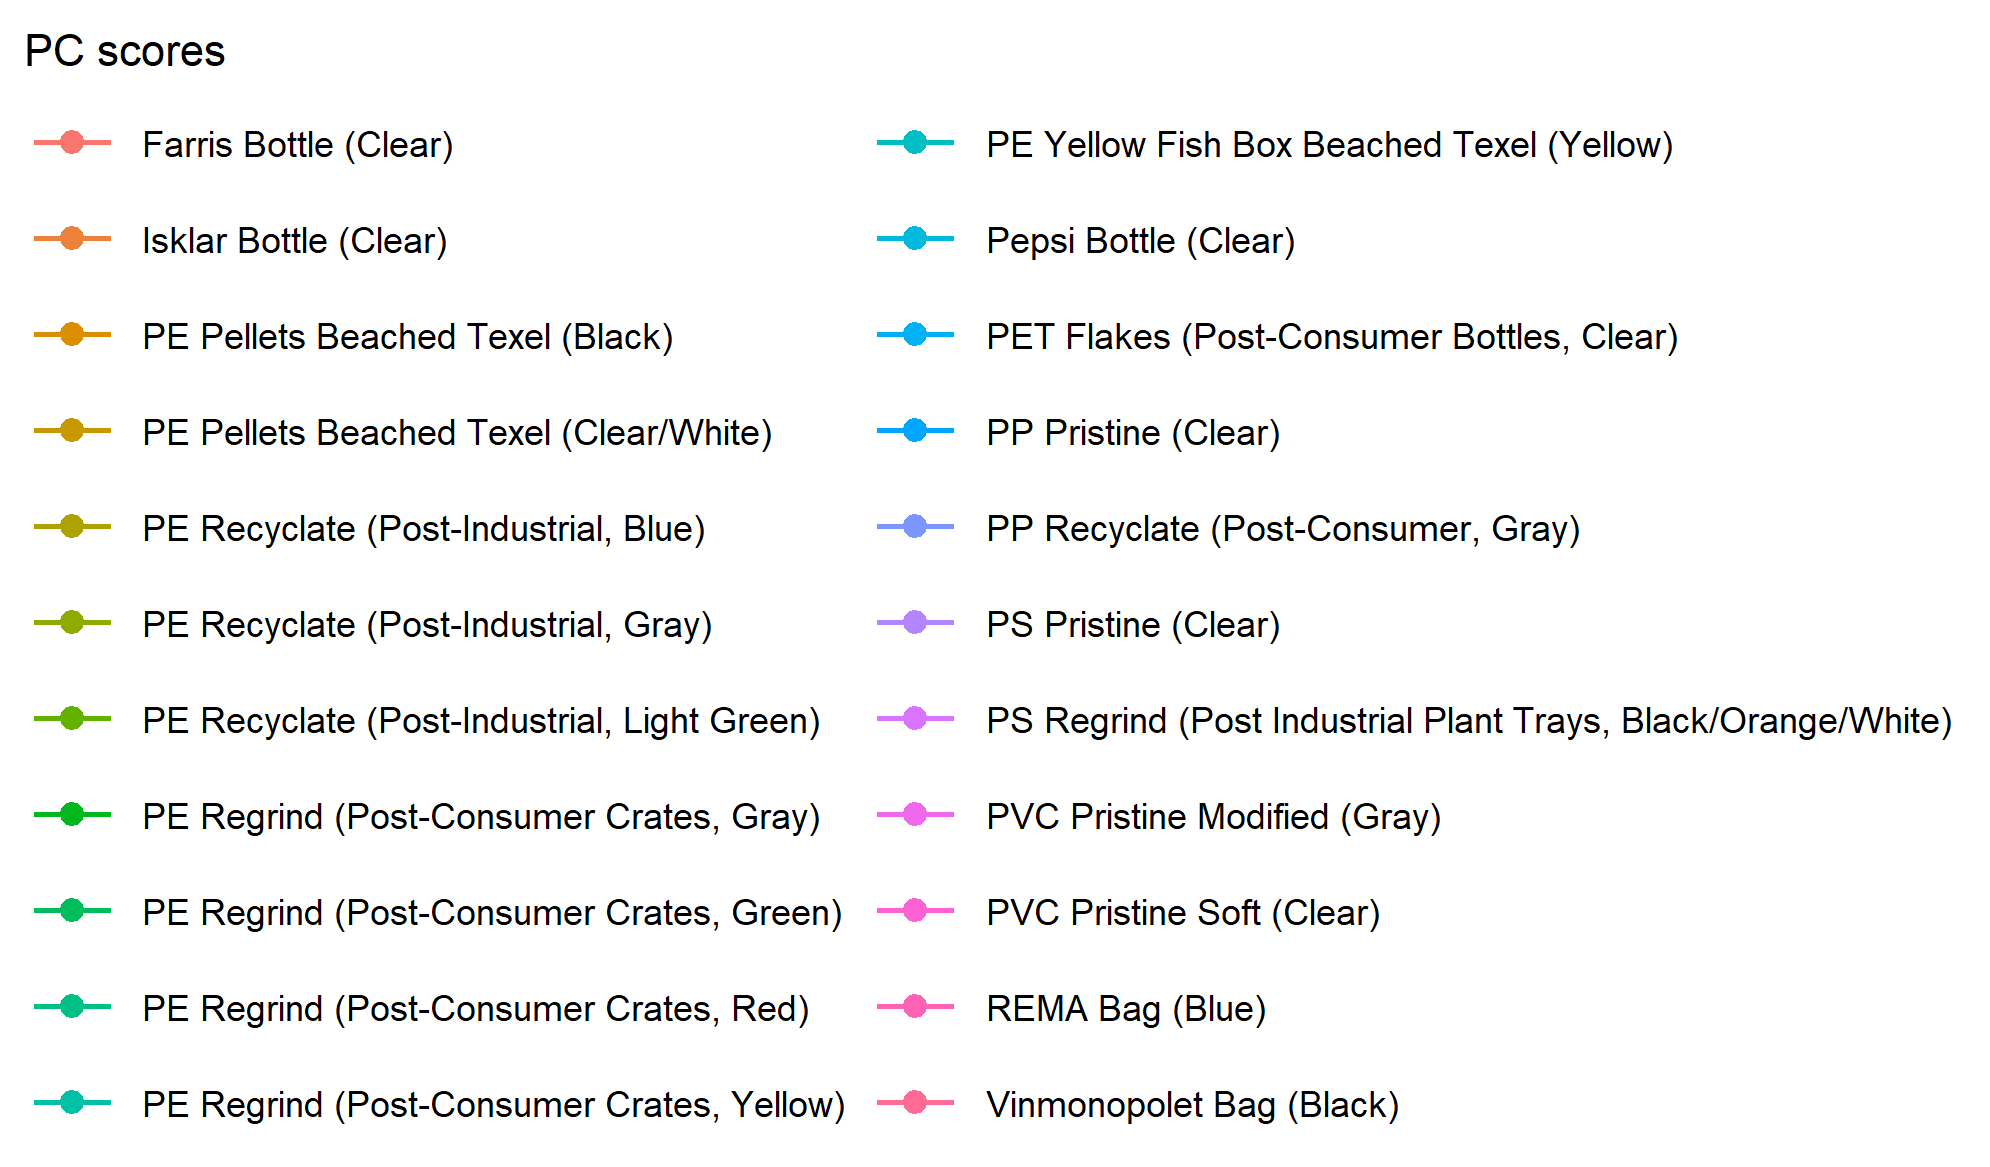
\includegraphics[width=0.7\textwidth]{Images/results/PCA_plastics_reduced_list.png}
    \caption{List of the reduced scanned plastic samples and their respective colors.}
    \label{fig:PCA_plastics_reduced_list}
\end{figure}

\begin{figure}[H]
    \centering
    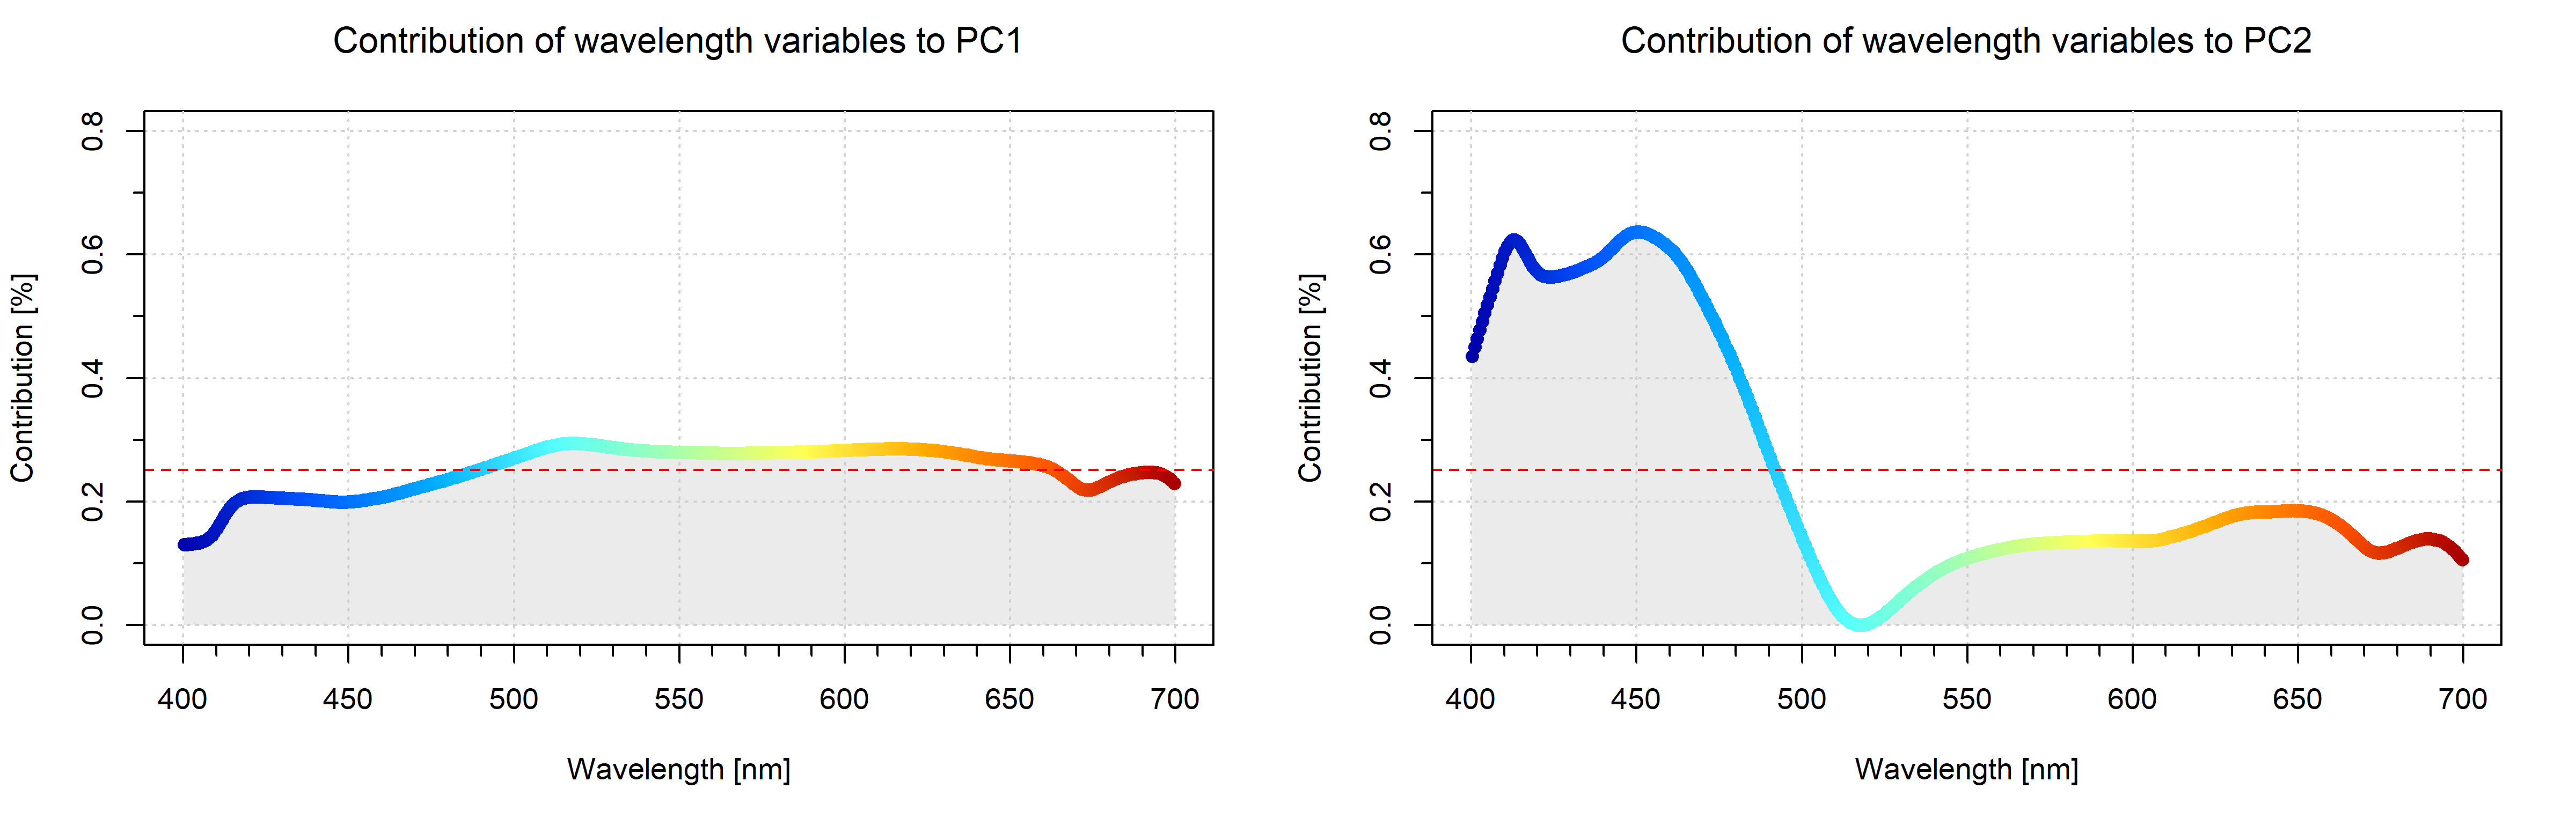
\includegraphics[width=1\textwidth]{Images/results/PCA_plastics_reduced_doub_cont.png}
    \caption{Contribution plots of the two principal components of the PCA with reduced plastic samples}
    \label{fig:PCA_plastics_doub_cont}
\end{figure}

\subsection{PCA with Biological Components}
When compared to results from testing on biological pigments, a more prominent trend became apparent. The natural occurring pigment in algae and crustaceans differed from the plastic in the scatter plot. This shows potential for distinguishing plastic in general from organic pigments naturally occurring in the marine environment.
\\\\%Argumentere med at her ser man at den klare plasten ligger utenfor konfidens intervallet og kan dermed mulig ekskluderes i en ny runde med forsøk, eventuelt at man endre bakgrunnen slik at den ikke er hvit og dermed ikke påvirker lysheten i tilsvarende grad. 
Below are plots with the same composition as those which solely contain plastic. The contribution on the first principal component does not differ much from that in the previous plots. However, given the aforementioned effect of the clear plastic, this might change with the use of a less reflective background. Furthermore, in figure \ref{fig:PCA_plastics_and_biology_scat} all plastic samples are gathered in one confidence interval ring. The clear result is that the previously mentioned clear plastic lies outside the confidence interval. This would further underline the previous suspicion that there is a prominent effect from the white background on the results.
\\\\
Experience has shown that the brightness/lightness of the samples is highly relevant also when not investigating plastic. Therefore, the change in background might affect the results, but it is not expected to revolutionize them.

\begin{figure}[H]
    \centering
    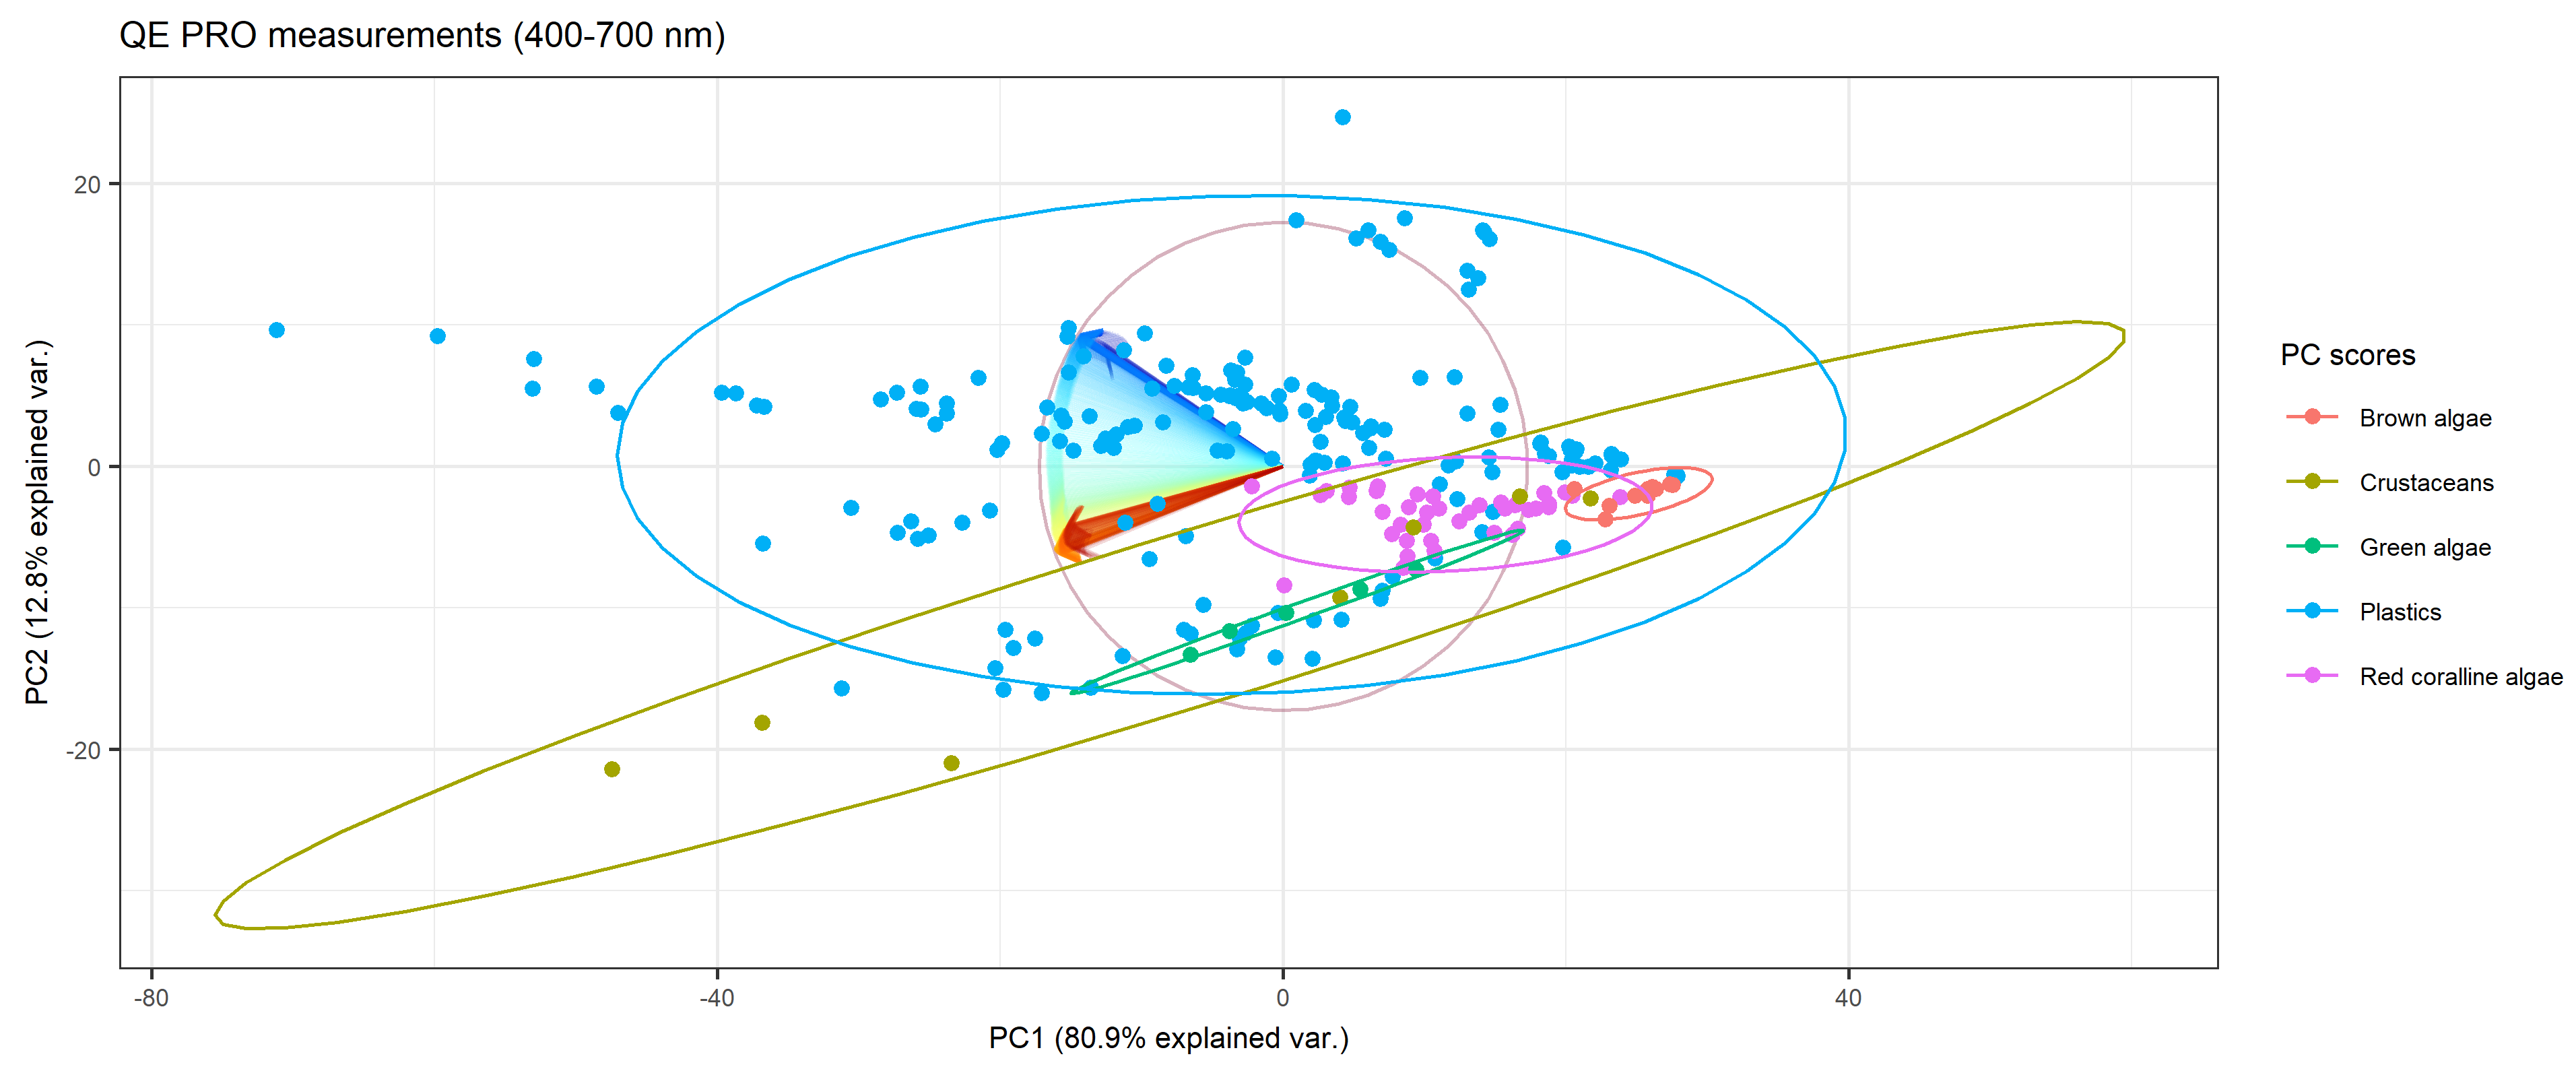
\includegraphics[width=1\textwidth]{Images/results/PCA_plastics_and_biology_scat_clust.png}
    \caption{Results of the PCA with Plastics and Biological Components}
    \label{fig:PCA_plastics_and_biology_scat}
\end{figure}

\begin{figure}[H]
\centering
\begin{subfigure}{.5\textwidth}
  \centering
  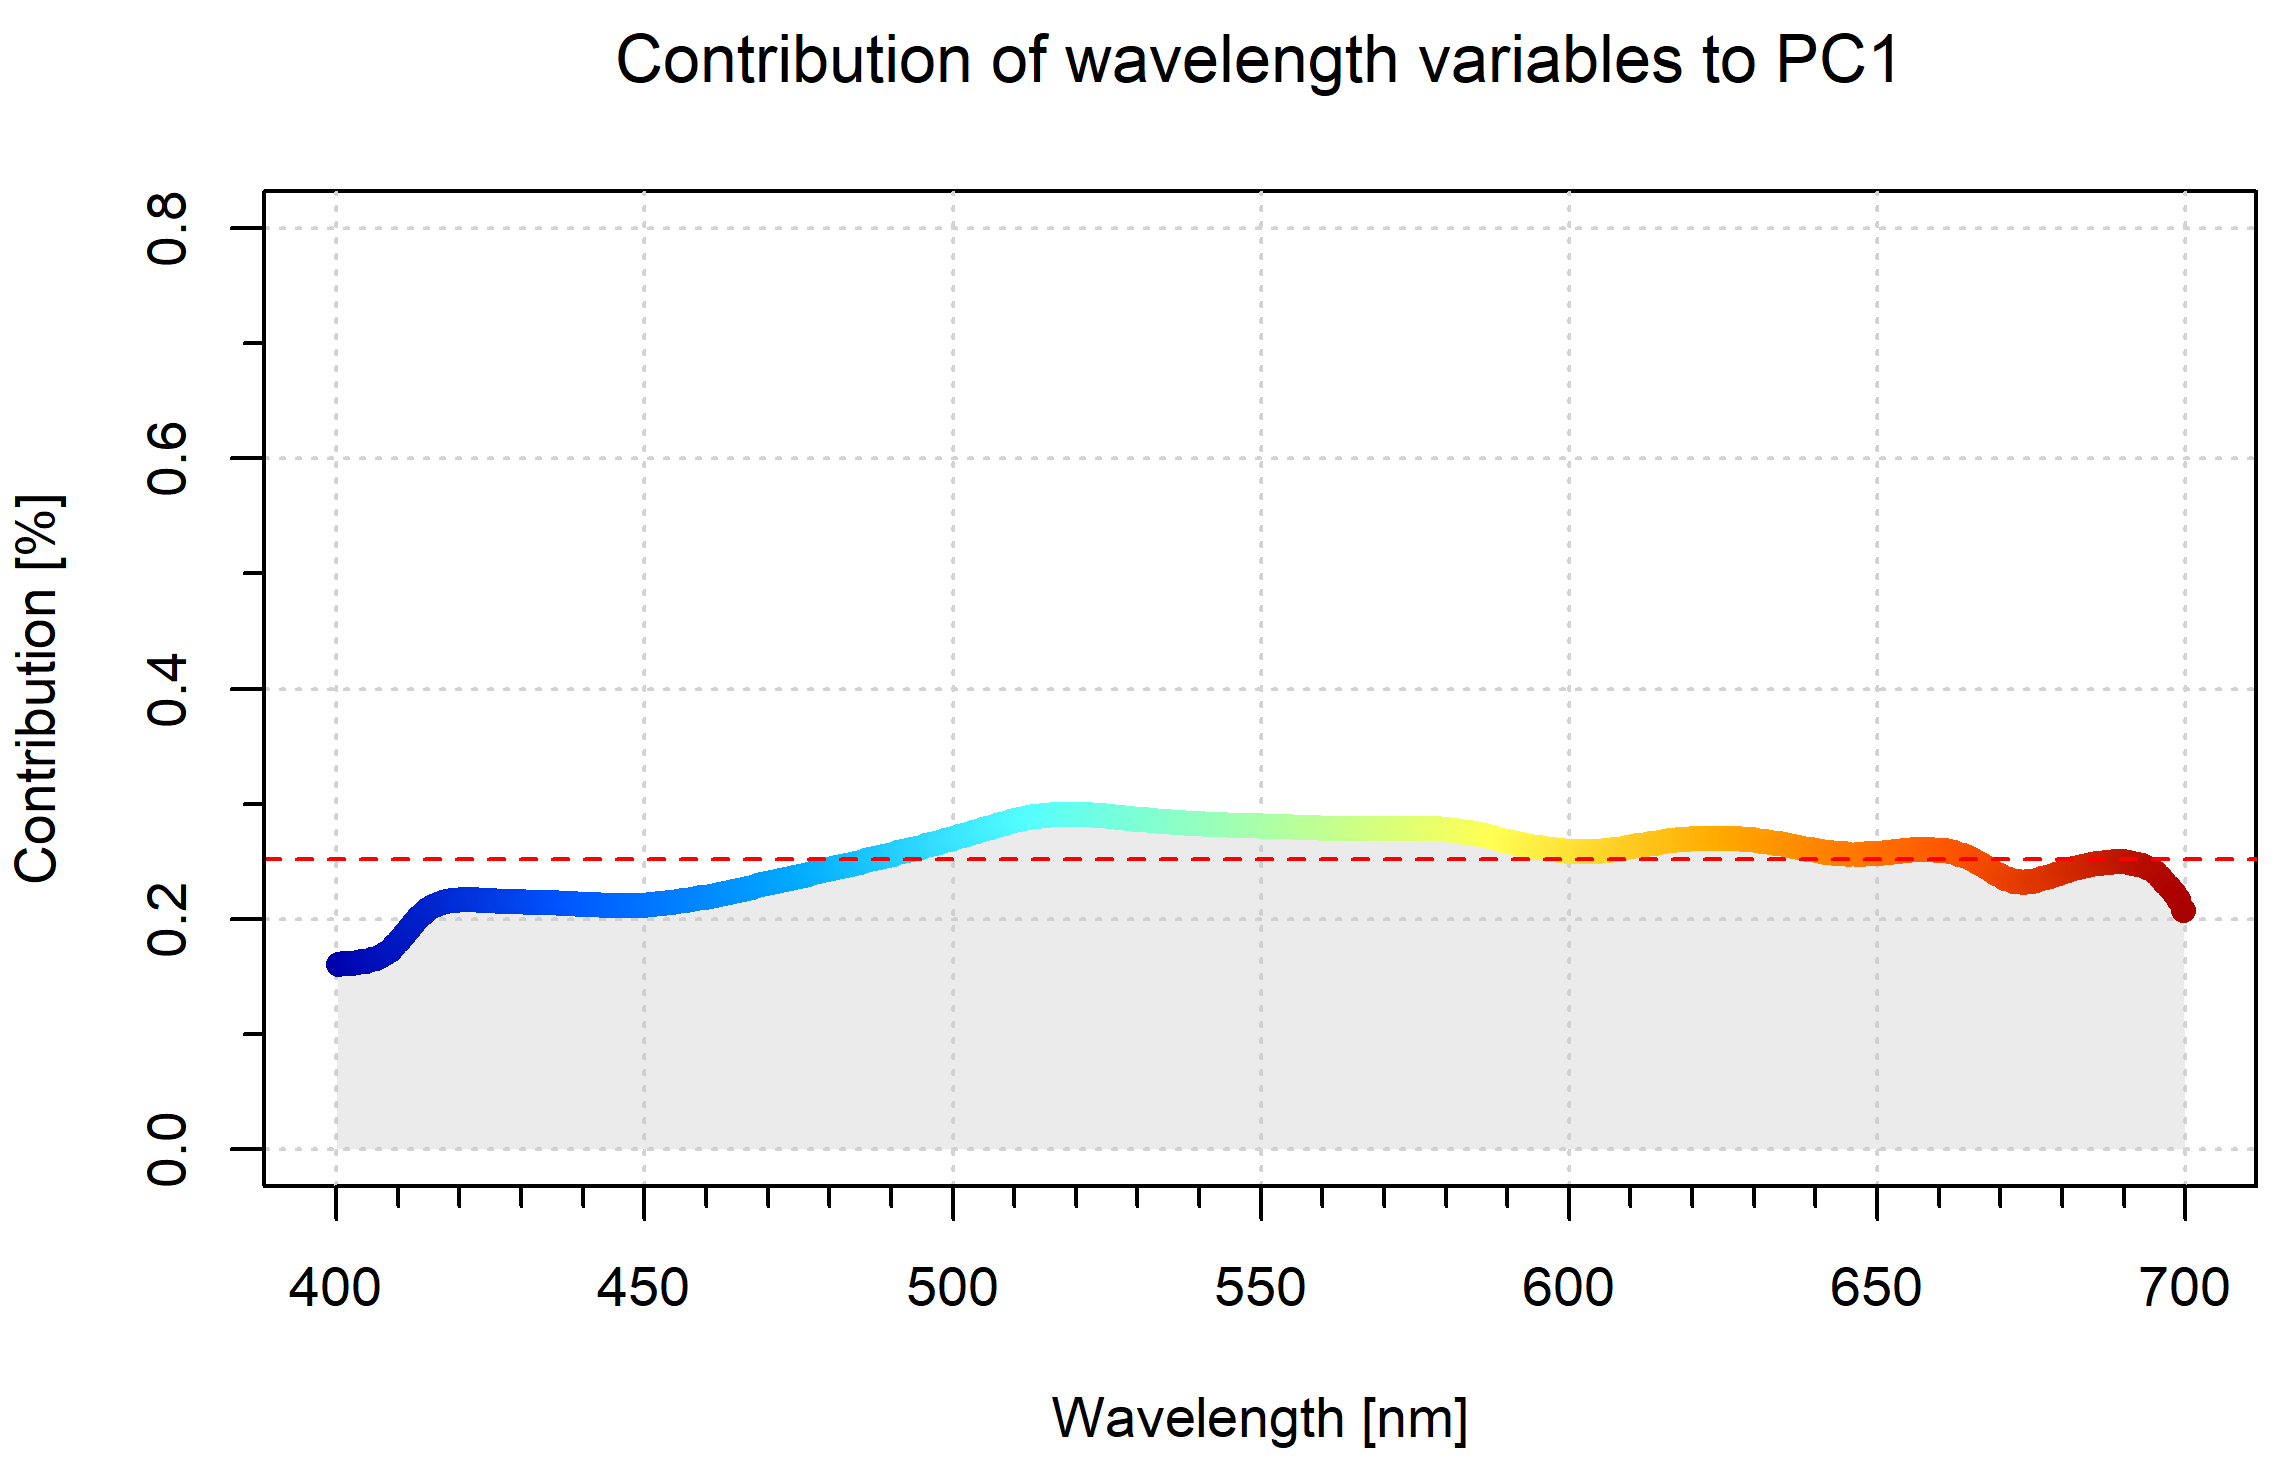
\includegraphics[width=\textwidth]{Images/results/PCA_plastics_and_biology_cont_pc1.png}
  \caption{Contribution plot of PC1}
  \label{fig:PCA_plastics_and_biology_cont_pc1}
\end{subfigure}%
\begin{subfigure}{.5\textwidth}
  \centering
  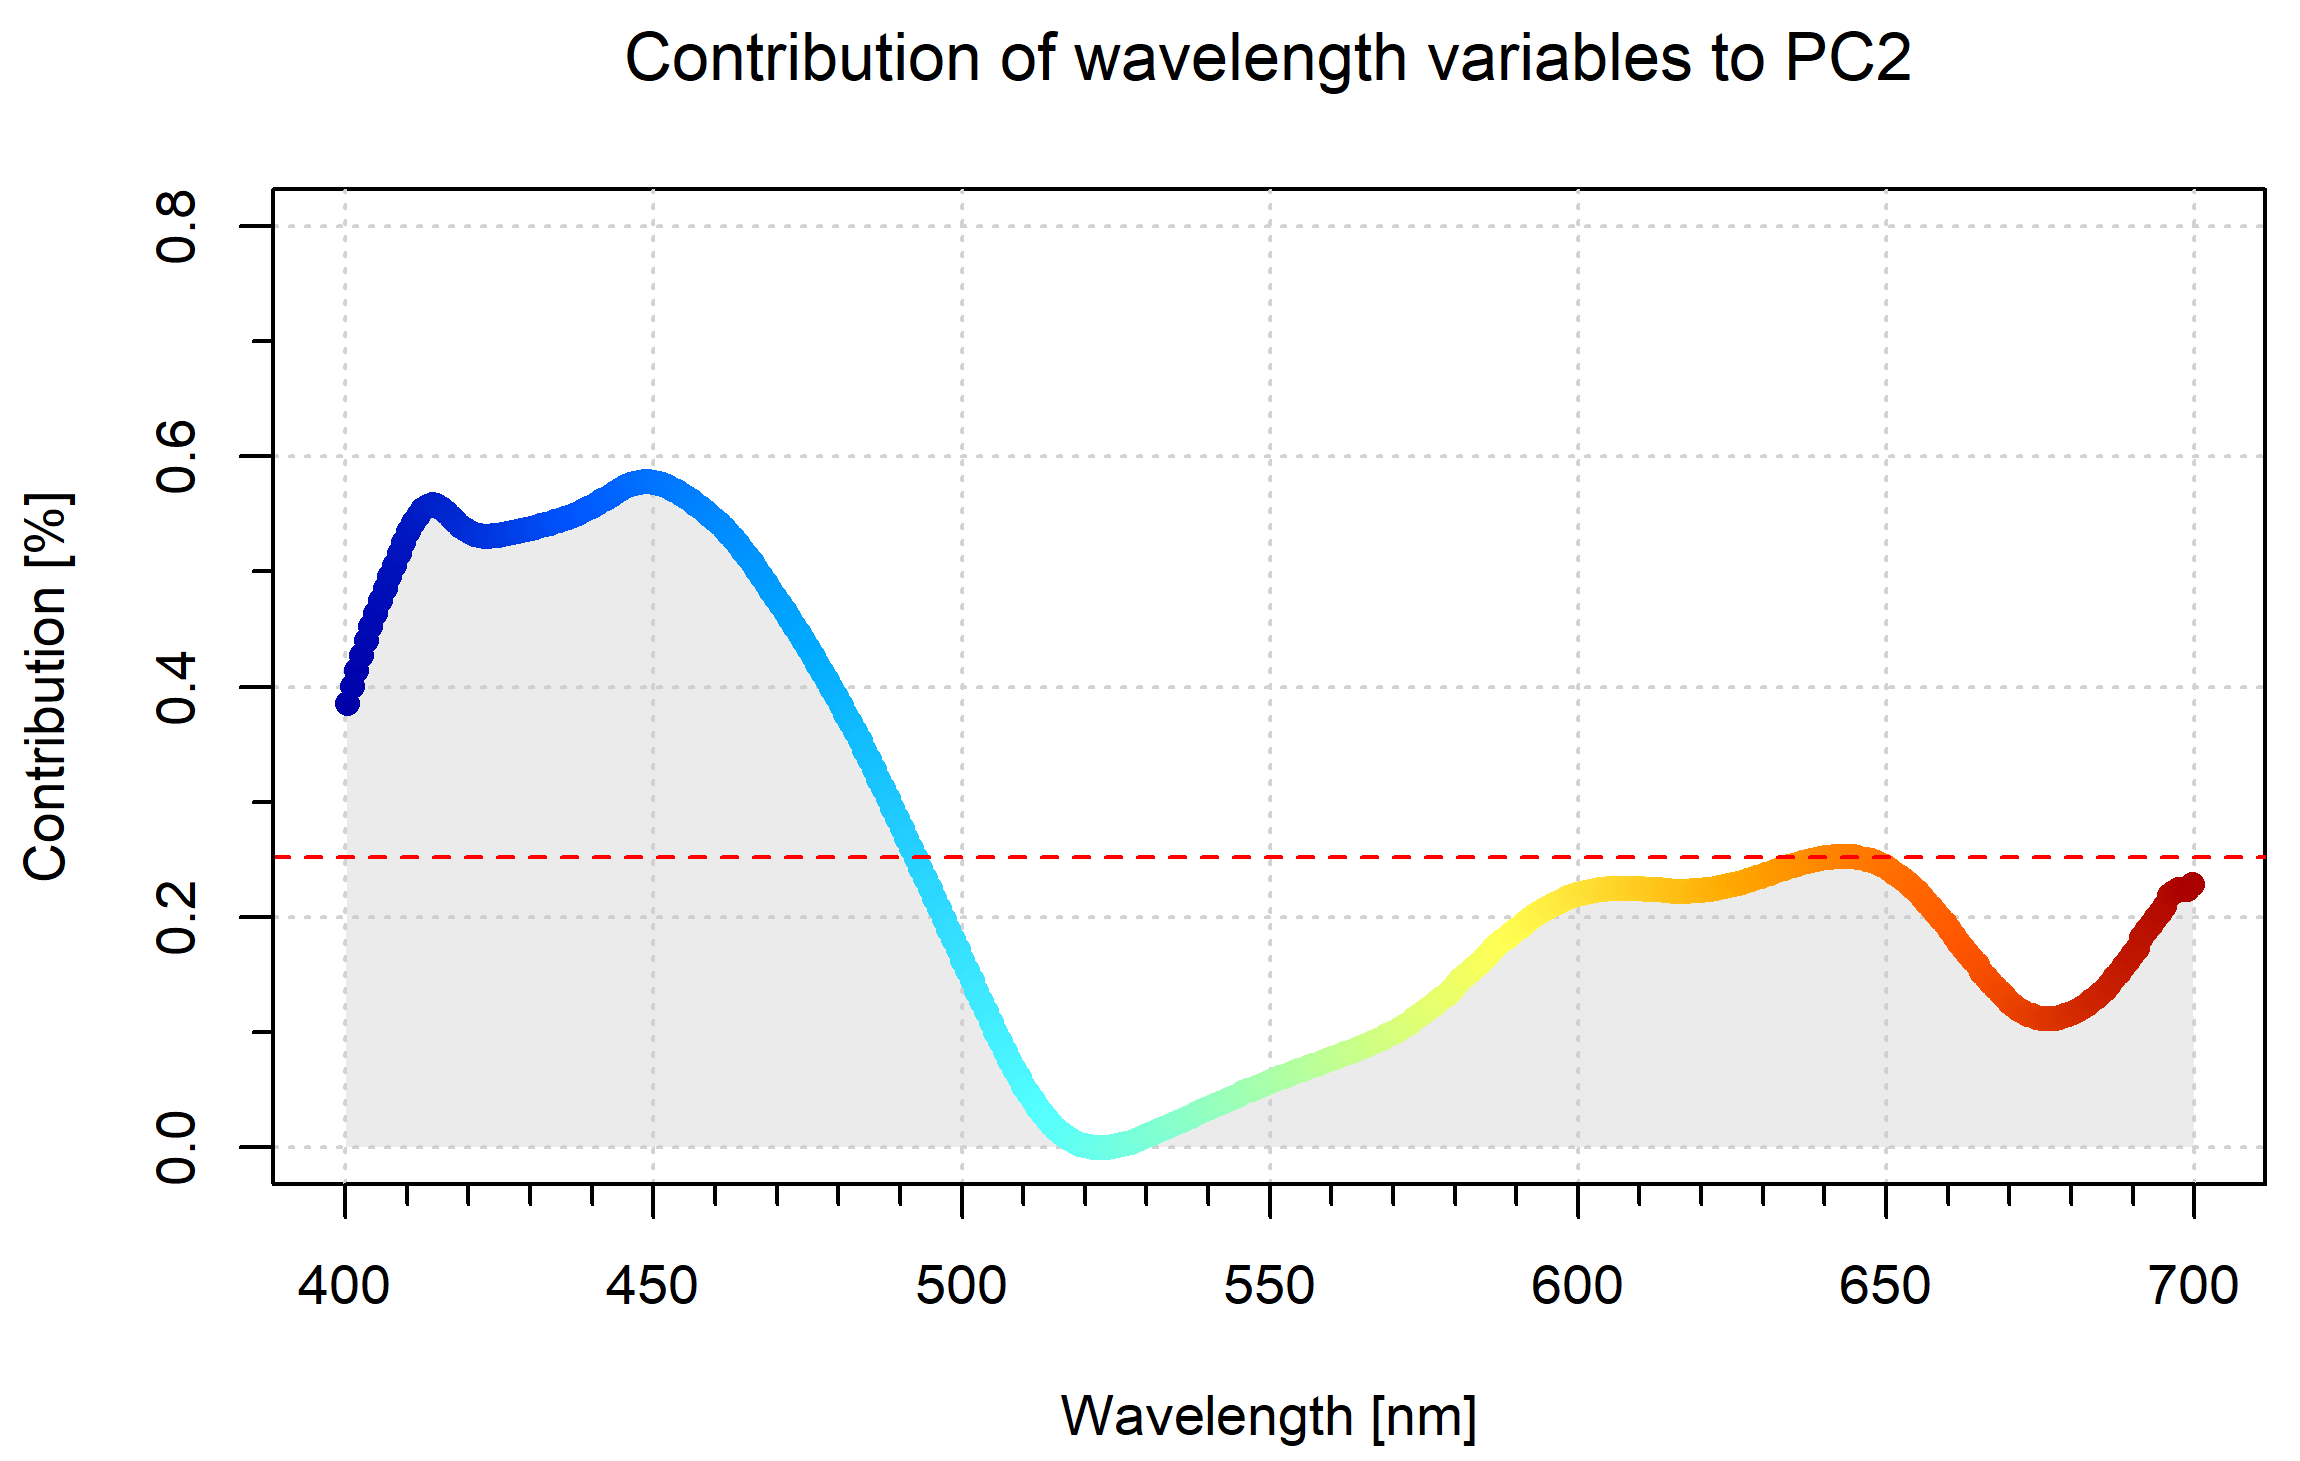
\includegraphics[width=\textwidth]{Images/results/PCA_plastics_and_biology_cont_pc2.png}
  \caption{Contribution plot of PC2}
  \label{fig:PCA_plastics_and_biology_cont_pc2}
\end{subfigure}
\caption{Contribution plots for the PCA with plastic and biological samples}
\label{fig:PCA_and_bio_cont_plots}
\end{figure}

\vspace{1.3cm}
\section{Signatures}
As previously mentioned, it was not possible to acquire distinct signatures for the individual types of plastic. Neither was is possible to find a general signature for the plastic which could be used as an end-member or for Spectral Angle Mapping. Despite seeing a resemblance of a signature in the second principal component it is important to keep in mind the components does not represent actual signatures. They rather depict the wavelengths which have a larger influence on the vertical distinguishing of the samples.
\\\\
Based on the absence of clear clusters it was deemed not possible to acquire signature for the plastic at this stage. All three analyses do show vertical spread, but the large number of overlapping samples made it difficult to argue for the existence of clear signatures at this stage. In the analysis with the presence of the organic pigments, there are some indication of separation, but not enough argue for a general signature for the plastic. However, the clustering seen in the sample does pose an opportunity of distinguishing plastic from the natural occurring pigments.